\documentclass[a4paper]{article}
\usepackage[utf8]{inputenc}
\usepackage{geometry}
\usepackage{amsmath}
\pdfpagewidth
\paperwidth
\pdfpageheight
\paperheight
\usepackage{booktabs}
\usepackage{graphicx}
\usepackage{subfig}
\usepackage{verbatim}
\newcommand*{\unit}[1]{\ensuremath{\mathrm{\,#1}}}
\usepackage{amsthm}
\usepackage{epsfig}
\usepackage{fancyhdr} 
\usepackage{amsmath,amssymb}
\usepackage{amscd} 
\usepackage[T1]{fontenc} 
\usepackage[utf8]{inputenc} 
\usepackage[usenames,dvipsnames]{xcolor}
\usepackage{graphicx,color,listings}
\usepackage{hologo}
\frenchspacing 
\usepackage{float}
\usepackage{geometry}
\usepackage{rotating}
\usepackage{caption}
\captionsetup{labelformat=empty, textfont=sl}
\usepackage{placeins}
\usepackage{hyperref}
\frenchspacing
\title{Esperienza Laboratorio di Fisica Medica: Rivelatori a semiconduttore (Si)}
\author{Simone Lossano, Lorenzo Marini, Jake Harold Pensavalle}
\begin{document}
	\maketitle
	\tableofcontents
	\newpage
	
	\section{Calibrazione segnali test}
Vogliamo anzitutto generare dei segnali per simulare lo spettro delle sorgenti radioattive che andremo ad analizzare, così da poter calibrare gli strumenti per le successive acquisizioni con rivelatore. Vengono così creati impulsi tramite il generatore di onde ed osservati attraverso un oscilloscopio multicanale. Infine, lo spettro simulato viene acquisito ed analizzato con un software ("\textbf{MAESTRO}") tramite una DC collegata all'oscilloscopio.  Tramite degli attenuatori modifichiamo le ampiezze dei segnali test, ottenendo le misure riportate nella tabella seguente, al fine di ottenere una calibrazione dell'oscilloscopio multicanale. Vogliamo cos\'i poter stimare i canali corrispondenti alle energie dei fotopicchi dell'Am-241 e del Cd-109 (60 keV, 22 keV). 
	\newline
	
	Come zero della scala del multicanale si imposta il \textbf{channel (Chn) 11}. I segnali test vengono inviati ad un condensatore test da C $\simeq$ 1 pF (in Si $E_{e-h}$ = 3.6 eV)
	
\begin{center} 
		
		\begin{tabular}{lccccccc}
			\hline
			\hline
			\textbf{ $\Delta$V} [mV]   &   Energy (keV)  	& \textbf{Attenuation} (dB)  &  \textbf{Chn}  &   \textbf{FWHM}  & \textbf{Gross Area}  & \textbf{Net Area}   	 \\
			\hline
			\hline
				      1.04                   & 23.4  &       43	(30+12+1)		        &      		85.58	&	1.69			&27810			&	26120 $\pm$ 11	\\
				       2.16                   &  48.6 &        38 (30+6+2)     			&		176.57  	&	1.69			&27809  			&	27809 $\pm$ 11\\
				       3.68		        &  82.8 &       33.5 (30+2+1+0.5) 			& 		305.20      & 	1.66			&27772 			&	 27772 $\pm$ 11\\
				       4.16		        & 93.6 &        32.5 (30+2+0.5)			& 		342.69 	& 	1.73			&27749			&	 27749 $\pm$ 11\\
			
			\hline
			\hline
		\end{tabular}
		\linebreak
		\emph{Tab.1: Dati di calibrazione: I canali e la FWHM sono relativi ai picchi osservati tramite il programma MAESTRO, cos\'i come la Gross Area e la Net Area.} 
	\end{center}

Tramite la relazione:

     \begin{equation}
     E(\Delta V) = {{C\Delta V}\over{e}} E_{e-h} 
     \end{equation}

abbiamo ricavato i valori di energia, inseriti nella tabella 1, al variare della tensione dei segnali in ingresso per poter ottenere la calibrazione Chn - Energy. 
Una volta ricavati i valori delle energie sono stati plottati in funzione dei valori dei canali corrispondenti (quest'ultimi ricavati tramite il software MAESTRO), procedendo con un fit per verificare la linearit\'a (Fig. 1).  
\newpage

\begin{figure}[!h]
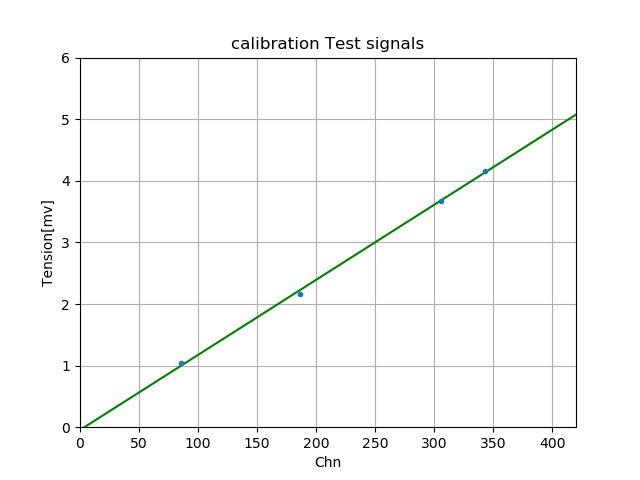
\includegraphics[width=1\textwidth]{calibration_test_signals}
        \caption{Fig. 1: Fit per la calibrazione dei segnali di test. I parametri stimati sono il coefficiente angolare $m$ = 0.271 $\pm$ 0.003, e l'intercetta \'e 0.352 $\pm$ 1.058.  }
        \label{fig:1}
\end{figure}

Invertendo la relazione, ricaviamo i valori attesi per i canali per i fotopicchi a 59.6 keV e 22.6 keV: \textbf{Chn(59.6keV) = 218.6}, \textbf{Chn(22.6keV) = 79.9}.
\newpage

Trovato il miglior setting dei parametri, studiamo come varia la risoluzione energetica in funzione dell'attenuazione del segnale (Gain). Tali valori sono ricavati a partire da quelli in Tabella 1. 

\begin{figure}[!h]
\includegraphics[width=1\textwidth]{Energy_vs_gain}
        \caption{Fig. 2: Fit per l'energia in funzione dell'attenuazione (gain) dell'ampiezza del segnale. Un'interpolazione di dati mostra come questi siano meglio fittati da una funzione cubica (valore di $R^2$ più vicino ad 1) del tipo $ax^3+bx^2+cx+d$, con $a=0.0000007 $, $b=-0.0000700 $, $c=0.0023323 $, $d=-0.259776 $ ed $R^2=1.000$}.
        \label{fig:2}
\end{figure}

\newpage

\section{Risoluzione energetica in funzione delle capacit\'a e valutazione del rumore del sistema}

Trovato il giusto setting dei parametri, abbiamo collegato al preamplificatore diversi cavetti LEMO (che serviranno a collegare il rivelatore al setup) che costituiscono delle capacit\'a. Utilizziamo un segnale di ampiezza \textbf{4.16 mV} (Tab.1) e lo testiamo per diversi valori 

\begin{center} 
		
		\begin{tabular}{lccccc}
			\hline
			\hline
			\textbf{Capacity} [pF]   &     \textbf{FWHM}         	&  \textbf{Chn}              &  \textbf{Energy} [KeV]  &   \textbf{Net Area}    	 \\
			\hline
			\hline
				       6.9                      & 1.72  			&       344.04			        &      		93.58	&	27660 $\pm$ 166						\\
				       27.1                   &  2.05 			&        344.46    			&	93.70	  	&	27666 $\pm$ 166			  			\\
				       18.6		        &  1.89 			&       345.31  			        & 		93.93      & 	27699 $\pm$ 166			 			\\
				       12.4		        & 1.76 			&        342.62 			      & 		93.17 	& 	27687 $\pm$ 166						\\
			    		?			&1.84			&	  346.00			       &		94.12	&	27701 $\pm$ 166							\\
			\hline
			\hline
		\end{tabular}
		\linebreak
		\emph{Tab.2: Dati di calibrazione: Il canale è relativo al picco osservati tramite il programma MAESTRO, cos\'i come la FWHM e la Net Area. Le energie sono state trovate tramite la funzione di calibrazione. Con "?" è indicata la capacità incognita.} 
	\end{center}
	
\begin{center} 
		
		\begin{tabular}{lcc}
			\hline
			\hline
			\textbf{Capacity} [pF]   &     \textbf{Energy Resolution} 	 \\
			\hline
			\hline
				       6.9              &	0.0183 \\
				       27.1             &	0.0219 \\
				       18.6		        &	0.0201 \\
				       12.4		        & 	0.0188 \\
			    		?			    &  	0.0196 \\
			\hline
			\hline
		\end{tabular}
		\linebreak
		\emph{Tab.3: Capacità vs risoluzione energetica, quest'ultima ottenuta utilizzando le energie dei picchi in Tabella 1} 
	\end{center} 	
	
L'interpolazione dei dati mostra come questi ultimi siano meglio fittati tramite una funzione quadratica.

\begin{figure}[!h]
\includegraphics[width=1\textwidth]{Capacity_vs_Resolution}
        \caption{Fig. 3: Fit per la risoluzione energetica in funzione della capacità. I punti sono meglio interpolati tramite una funzione del tipo $ax^2+bx+c$. I valori stimati dei coefficienti sono: $a = 0.0000037$, $b = 0.000053$, $c = 0.017$, con $R^2 = 0.991$.}
        \label{fig:3}
\end{figure}

\newpage

Dal fit possiamo così stimare il valore della capacità incognita tramite la risoluzione energetica, che risulta essere pari a \textbf{16.533 pF}.


Per quanto riguarda la valutazione del rumore introdotto dalla capacità sul segnale, sappiamo che:

     \begin{equation}
     FWHM_{tot}^2=FWHM_{stat}^2+FWHM_{noise}^2+FWHM_{drift}^2
     \end{equation}
     
Avendo eseguito nuovamente le misure dopo un ragionevole intervallo di tempo, notiamo dal programma MAESTRO che non ci sono cambiamenti apprezzabili della posizione del picco, per cui possiamo supporre la componente di \emph{drift} del rumore $\simeq 0$.
Avendo utilizzato sempre lo stesso segnale in ingresso, possiamo supporre che la $FWHM_{stat}^2$ sia costante (1,73), quindi, avendo precedentemente analizzato l'andamento della risoluzione energetica in funzione della capacità, possiamo supporre inoltre che la $\sigma_{noise}$ presenti circa lo stesso andamento in funzione della capacità, a meno di una costante additiva. Infatti, ogni altra componente alla risoluzione oltre la $FWHM_{noise}$ per i punti in Fig.4, rimane la stessa.

\section{Studio dello spettro di sorgenti radioattive $\gamma$.}
Abbiamo due tipi di sorgenti radioattive a disposizione: \textbf{241-Am} e \textbf{109-Cd}. 

\subsection{Americio}
Anzitutto colleghiamo il rivelatore (quello fornitoci è contrassegnato come \textbf{n.o 4}) al preamplificatore, scolleghiamo il generatore d'onde e, successivamente, procediamo a piazzare dentro un apposito foro nel rivelatore la sorgente di \textit{241-Am}.  Trattandosi di una giunzione p-n, cerchiamo il valore ottimale di tensione da fornire allo strumento affinchè sia in regime di sovrasvuotamento. 
\\

Facciamo una prima acquisizione dello spettro con una tensione di 4.0 V, notiamo che in corrispondenza del supposto picco a 59.6 KeV se ne presentano invece due ravvicinati (Fig. 4, sotto). Il motivo sembra essere che il valore della tensione scelto non sia sufficiente affinchè la larghezza della zona di svuotamento sia tale da far sì che l'intera carica di ionizzazione prodotta dai fotoni emessi dalla sorgente venga raccolta.

\begin{figure}[!h]
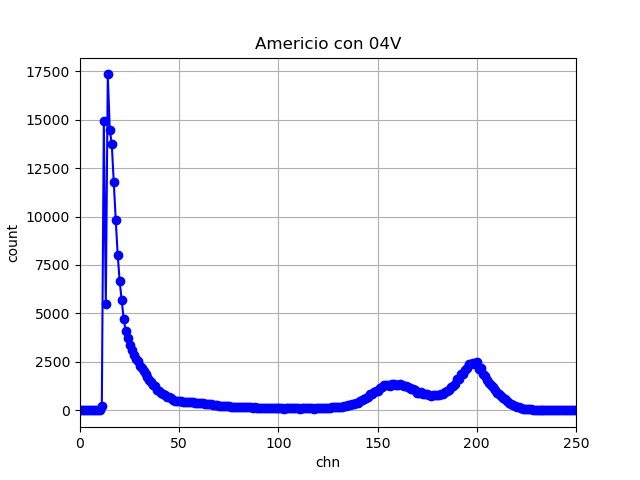
\includegraphics[width=1\textwidth]{Americio_con_04V}
        \caption{Fig. 4: Spettro dell'Americio con tensione 4.0V. Si notano due picchi ravvicinati in corrispondenza della zona dove ci                                     						 aspetteremmo il fotopicco a causa del valore di tensione di svuotamento troppo basso.}
        \label{fig:4}
\end{figure}

Viene quindi osservato il fotopicco dell'Americio per diversi valori di tensione (riportati in Tab.4) per cercare quella di lavoro (cioè una in cui ci sia sovrasvuotamento della regione di carica spaziale).
      
\begin{figure}[!h]
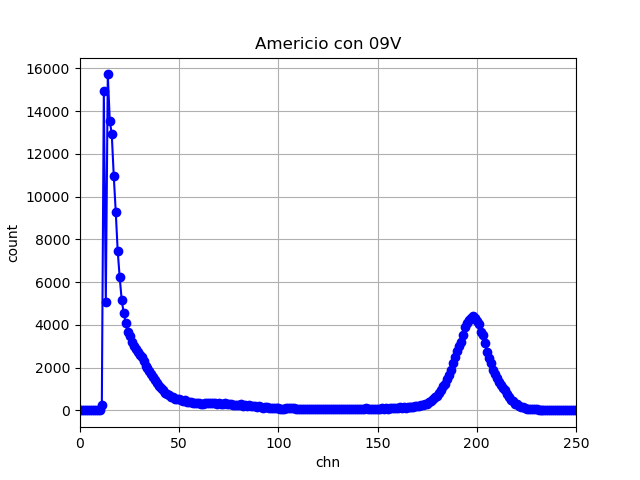
\includegraphics[width=0.5\textwidth]{Americio_con_09V}
        \caption{Fig. 5: Spettro dell'Americio con tensione 9.0V. .}
        \label{fig:5}

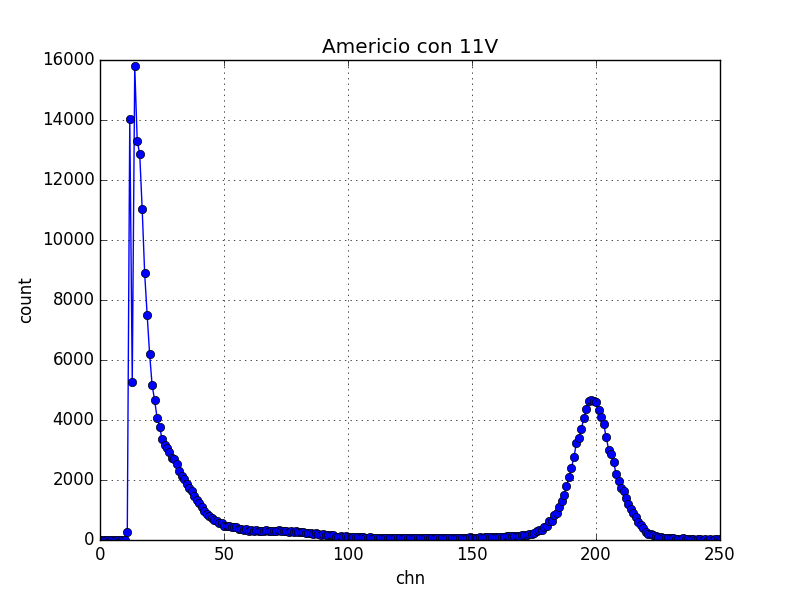
\includegraphics[width=0.5\textwidth]{Americio_con_11V}
        \caption{Fig. 6: Spettro dell'Americio con tensione 11.0V. .}
        \label{fig:6}

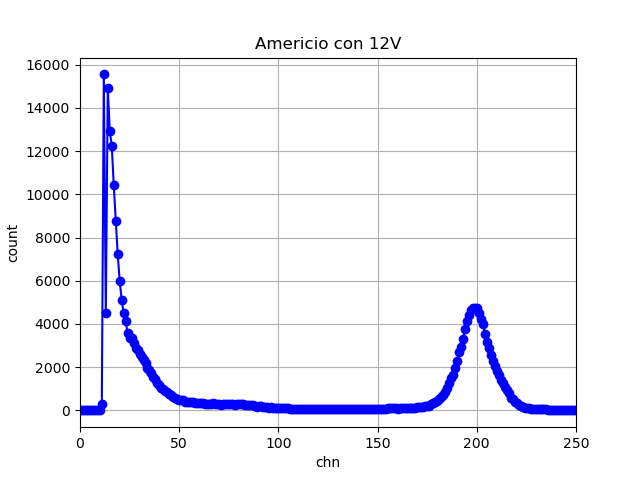
\includegraphics[width=0.5\textwidth]{Americio_con_12V}
        \caption{Fig. 7: Spettro dell'Americio con tensione 12.0V. .}
        \label{fig:7}
\end{figure}  
\newpage
	sdfghjklxcvbnm,xcvbnm,dfghjkcvbnm,


\begin{center} 
		
		\begin{tabular}{lccccc}
			\hline
			\hline
			\textbf{$\Delta V$} [V]   &     \textbf{Chn}		&     \textbf{Energy} [KeV]		&     \textbf{FWHM}		&     \textbf{Net Area} 	 \\
			\hline
			\hline
				       4.0             &	198.94			&		54.26			&				3.25		&			54727 $\pm$ 398\\
				       9.0             &	197.64 			&		53.91			&				3.89		&			91390 $\pm$ 399\\
				       11.0		        &	198.97 			&		54.27			&				3.60		&			92393 $\pm$ 393\\
				       12.0		        & 	198.85 			&		54.24			&				3.56		&			91896 $\pm$ 397\\
			\hline
			\hline
		\end{tabular}
		\linebreak
		
		\emph{Tab.4: Dati del fotopicco dell'Americio a diverse tensioni di svuotamento del rivelatore. L'energia del picco è 							 stata trovata tramite la funzione di calibrazione ricavata precedentemente. La FWHM è ricavata da MAESTRO. Per la tensione a 4.0V, viene preso in considerazione solo il picco al Chn 198. } 
	\end{center} 	
\'E anzitutto evidente che l'energia ottenuta dalle acquisizioni per il fotopicco dell'Americio non sia quella attesa. Tale discrepanza è possibile ricordando che il rivelatore è dotato di una capacità interna che non conosciamo. 
Possiamo notare però che per valori di tensione intorno ai \emph{12 V}, la posizione del picco e la Net Area sono circa costanti. \'E ragionevole pensare perciò che siamo in condizione di sovrasvuotamento, scegliamo quindi come tensione di lavoro \textbf{12 V}.
\\

Abbiamo quindi proceduto nell'analizzare i picchi con un fit gaussiano dei dati, dai quali abbiamo successivamente ricavato i valori di \emph{<x>} (Chn medio) e $\sigma$ riportati in Tab.5.

\begin{figure}[!h]
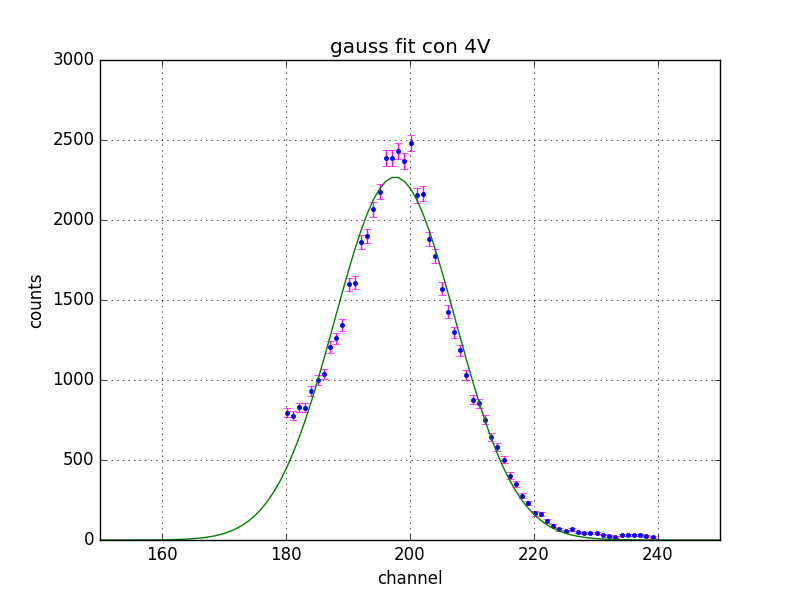
\includegraphics[width=0.3\textwidth]{Fit_Gaussiano_con_4V}
        \caption{Fig. 8: Fit Gaussiano del picco a 4.0 V. In questo caso viene analizzato solo il picco al Chn 198.}
        \label{fig:8}
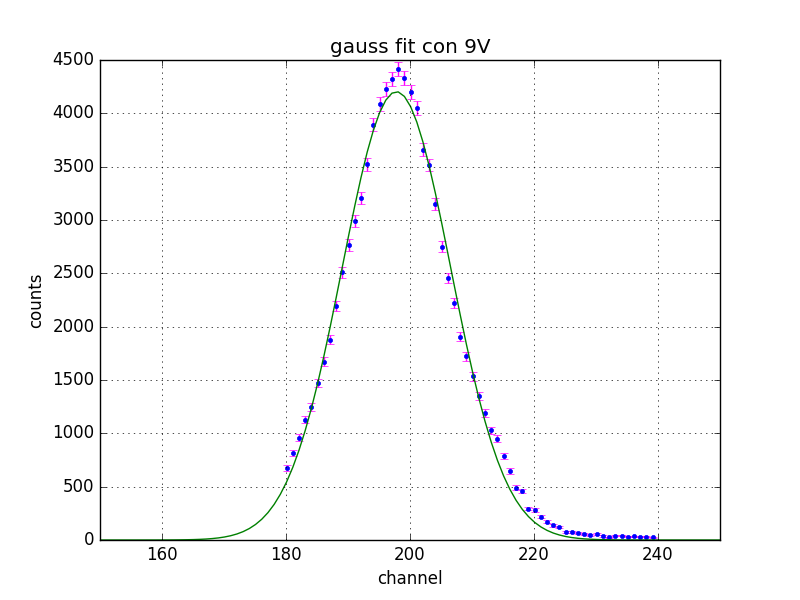
\includegraphics[width=0.3\textwidth]{Fit_Gaussiano_con_9V}
        \caption{Fig. 9: Fit Gaussiano del picco a 9.0 V}
        \label{fig:9}

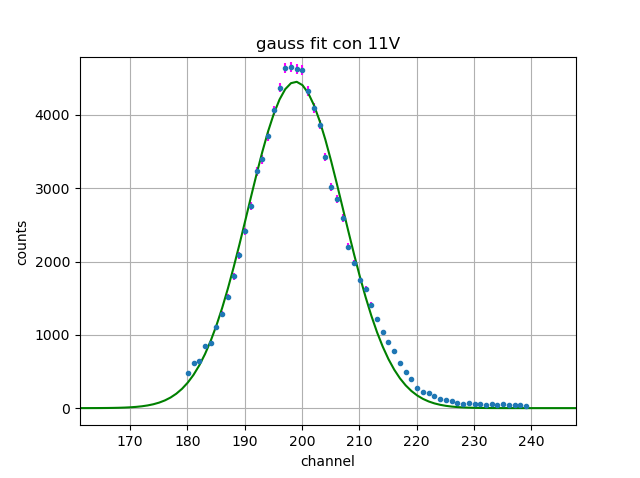
\includegraphics[width=0.3\textwidth]{Fit_Gaussiano_con_11V}
        \caption{Fig. 10: Fit Gaussiano del picco a 11.0 V}
        \label{fig:10}
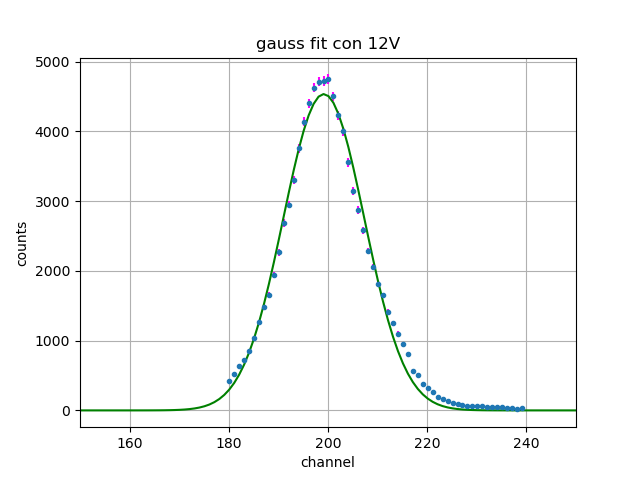
\includegraphics[width=0.3\textwidth]{Fit_Gaussiano_con_12V}
        \caption{Fig. 11: Fit Gaussiano del picco a 12.0 V}
        \label{fig:11}        
\end{figure}
\newpage

\begin{center} 
		
		\begin{tabular}{lcccc}
			\hline
			\hline
			\textbf{$\Delta V/V$} [V]   &     \textbf{$\sigma$}	 &     \textbf{<x>} &     \textbf{FWHM} & \textbf{$\Delta E/E$}	 \\
			\hline
			\hline
				       4.0              &		9.73			 &		197.59		&		 22.86	& 	0.115		\\
				       9.0             &		8.33			 &		198.88			&	 19.56	&	0.098 	\\
				       11.0		        &		8.17			 &		199.15			&	 19.20	&	0.096 		\\
				       12.0		        & 		8.76			 &		197.81			&	 20.59	&	0.104	 	\\
			\hline
			\hline
		\end{tabular}
		\linebreak
		\emph{Tab.5: Dati ottenuti dai fit gaussiani dei fotopicchi. Notiamo come ci sia una notevole discrepanza con i valori della FWHM in Tab.4. In particolare, quelli ottenuti tramite fit gaussiano, con una stima ad occhio dai grafici, sembrano essere quelli corretti. } 
	\end{center}
	
Dai dati così ottenuti, plottiamo la FWHM e <x> in funzione della tensione di svuotamento.

\begin{figure}[!h]
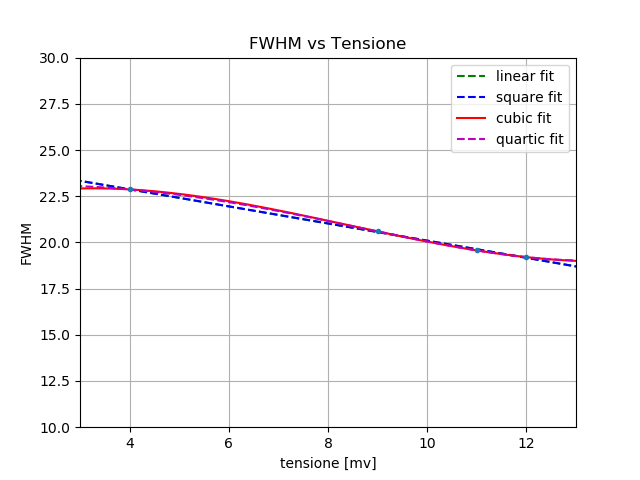
\includegraphics[width=1\textwidth]{FWHM_vs_Tensione}
        \caption{Fig. 12: FWHM in funzione tensione di svuotamento. Si vede che i punti sono meglio fittati tramite una funzione cubica del tipo $ax^3+bx^2+cx+d$, con coefficienti $a=0.057$, $b=-1.298$, $c=8.642$, $d=5.425$, $R^2= 1.000$.}
        \label{fig:12}
\end{figure}

\begin{figure}[!h]
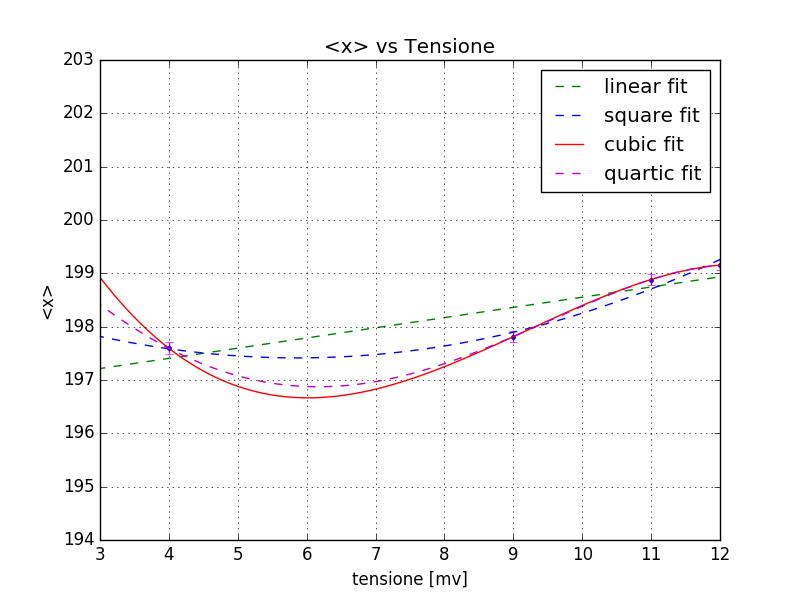
\includegraphics[width=1\textwidth]{x_vs_Tensione}
        \caption{Fig. 13: <x> in funzione della tensione di svuotamento. Si vede che i punti sono meglio fittati tramite una funzione cubica del tipo $ax^3+bx^2+cx+d$, con coefficienti $a=0.039$, $b=-1.407$, $c=-10.136$, $d=219.429$, $R^2= 1.000$}
        \label{fig:13}
\end{figure}
\newpage

\subsection{Cadmio}
In letteratura troviamo che il Cadmio presenta tre picchi: a 22.1 KeV, 25 KeV, 88KeV. Lavoriamo sempre alla tensione di svuotamento scelta per il rivelatore, cioè \textbf{12V} e per un tempo di acquisizione di \textbf{900s}. Dallo spettro visualizzato tramite MAESTRO, appare distinguibile un solo picco in corrispondenza del Chn 74, dove supponiamo i primi due picchi si siano sovrapposti, con il secondo che appare come una gobba sul picco a 22.1 KeV. Il picco a 88 KeV è invece assente poichè il tempo di acquisizione è insufficiente per avere una statistica apprezzabile.  
\begin{center} 
		
		\begin{tabular}{lcccc}
			\hline
			\hline
			\textbf{Chn}      &     \textbf{Energy} [KeV]  &     \textbf{FWHM} &     \textbf{Net Area} 	 \\
			\hline
			\hline
				      74.90  &	15.50	&		2.18 		& 2635 $\pm$ 59			\\
				       
			\hline
			\hline
		\end{tabular}
		\linebreak
		\emph{Tab.6: Dati del picco del Cadmio visualizzati tramite MAESTRO.} 
	\end{center} 	
Eseguiamo un fit gaussiano del picco ed otteniamo i seguenti dati:

\begin{center} 
		
		\begin{tabular}{lccccc}
			\hline
			\hline
			\textbf{Chn} & \textbf{$\sigma$}  &     \textbf{Energy} [KeV]  &     \textbf{FWHM}  & \textbf{Risoluzione Energetica}   & \textbf{Net Area} 	 \\
			\hline
			\hline
				       75.13   & 4.58(?)           &	20.71 $\pm$	&		10.76(?) & 0.52		& 2557 $\pm$ 59			\\
				       
			\hline
			\hline
		\end{tabular}
		\linebreak
		\emph{Tab.7: Dati del picco del Cadmio ottenuti tramite il fit gaussiano.} 
	\end{center}
	
\begin{figure}[!h]
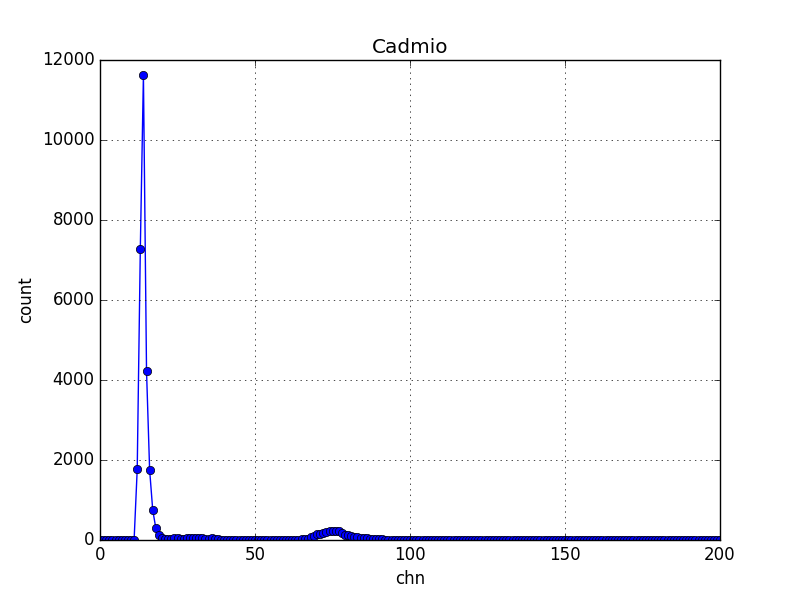
\includegraphics[width=0.8\textwidth]{cadmio.png}
        \caption{Fig. 14: Spettro del Cadmio, tempo di acquisizione 900s.}
        \label{fig:14}
\end{figure}7
\begin{figure}[!h]
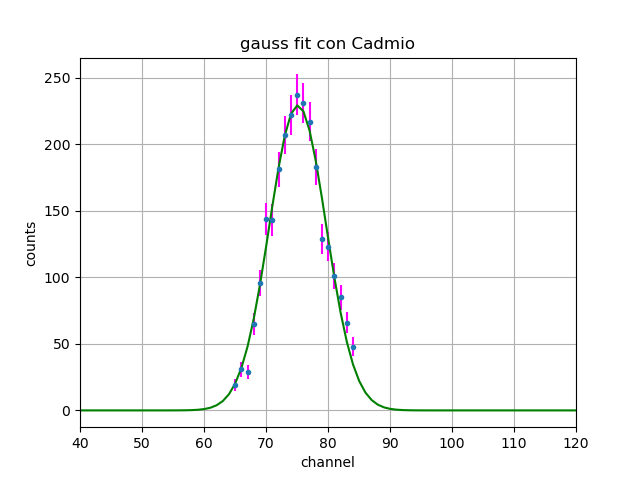
\includegraphics[width=0.8\textwidth]{fit_gaussiano_con_Cadmio.png}
        \caption{Fig. 15: Fit gaussiano del fotopicco del Cadmio.}
        \label{fig:15}
\end{figure}
\subsection{Calibrazione delle sorgenti e studio dello spettro con spessori.}

Dalle misure delle energie dei picchi acquisite dagli spettri dell'Americio e del Cadmio, vogliamo ottenere una nuova calibrazione Energy-Chn. Abbiamo però a disposizione solo due punti, per trovarne altri, che permettano di ottenere un fit, ricerchiamo altri picchi frapponendo tra la sorgente e il rivelatore lamine di vari materiali. Abbiamo a nostra disposizione:
\begin{itemize}
\item Gadolinio, spessore: $120 \mu m$
\item Gadolinio impuro, $100 \mu m$
\item Molibdeno, $50 \mu n$, $100 \mu m$
\item Stagno, $125 \mu m$
\item Nichel, $20 \mu m$
\end{itemize}




In letteratura sono note le energie dei fotoelettroni delle principali linee di emissione delle shell K,L ed M [rif. Radiation Detection and Measurements, G.F. Knoll].
 Ci aspettiamo così di vedere almeno il picco \textbf{$K_{\alpha_{1}}$} che si ottiene frapponendo questi materiali, oltre che il fotopicco, normalmente a 60 KeV, dell'Americio. \\
Lavoriamo sempre con una tensione di 12V sul rivelatore e il tempo d'acquisizione è fissato a \textbf{120 s}. Per ogni spessore viene riportato lo spettro ottenuto dai dati, vengono eseguiti i fit gaussiani dei nuovi picchi presenti sullo spettro e del fotopicco dell'Americio. I risultati sono raccolti nelle tabelle sottostanti.

$\#$QUI VANNO INSERITI I GRAFICI DEGLI SPETTRI DEGLI ELEMENTI CON LA TABELLA DATI DEI VARI FIT GAUSSIANI + LA CALIBRAZIONE CON I DATI DEL FIT. INFINE VA INSERITA UNA TABELLA IN CUI SI METTONO LE ENERGIE TROVATE CON LA FUNZIONE DI CALIBRAZIONE, QUELLE NOTE IN LETTERATURA E POI FWHM, ENERGIA DEL PICCO, NET AREA PER IL FOTOPICCO DELL'AMERICIO (QUEST'ULTIMA PER IL CONFRONTO DI COME CAMBIA LO SPETTRO DELL'AMERICIO).
\subsection{Attenuazione in un materiale}
Vogliamo valutare la legge di attenuazione in un materiale:
\begin{equation}
I=I_{0}e^{-\mu x}
\end{equation}
Utilizzeremo degli spessori di rame da \textbf{600 $\mu m$}, posizionati in modo da formare uno spessore crescente tra la sorgente di Americio e il rivelatore con tempi di acquisizione di \textbf{60 s}. Viene preventivamente fatta un'acquisizione della sola sorgente per valutare eventuali cambiamenti rispetto alle misure iniziali, non si osservano sostanziali variazioni.\\

Riportiamo i valori dei picchi osservati tramite MAESTRO e successivamente quelli ottenuti dal fit gaussiano.

\begin{center} 
		
		\begin{tabular}{lccccc}
			\hline
			\hline
			\textbf{N.o spessori} & \textbf{Chn}  &   \textbf{FWHM}   & \textbf{Net Area}	\\
			\hline
			\hline
				      1 &  201.36   & 2.38  &  27259	$pm$	215	\\
				      2 &  202.24   & 2.20	&  14953	$pm$	142 \\
				      3 &  202.74	& 2.09	&  7842		$pm$	111 \\
				      4 &  202.88	& 1.83	&  3967	$pm$	67 \\
				      5 &  203.17	& 1.94	&  1889	$pm$	47 \\
				      6 &  202.62	& 1.88	&  904	$pm$	33 \\
				      7 &  203.10	& 1.15	&  446	$pm$	24 \\
				      8 &  202.23	& 1.03	&  236	$pm$	16 \\
				      9 &  200.17	& 0.26	&  124	$pm$	12 \\
				      10 & 204.23	& 0.83	&  66	$pm$	8 \\
			\hline
			\hline
		\end{tabular}
		\linebreak
		\emph{Tab.8: Dati ottenuti tramite MAESTRO del picco dell'Americio a diversi spessori di Cu.} 
	\end{center}
 Riportiamo di seguito a titolo esemplificativo alcuni grafici estratti dall'analisi dati.
 
 \begin{figure}[!h]
\includegraphics[width=0.5\textwidth]{Visuale_a_Am0Cu}
        \caption{Fig. 8: Fit Gaussiano del picco senza spessori.}
        \label{fig:16}
\includegraphics[width=0.5\textwidth]{Visuale_a_Am3Cu}
        \caption{Fig. 9: Fit Gaussiano del picco con 3 spessori}
        \label{fig:17}
\end{figure}
\begin{figure}[!h]
\includegraphics[width=0.5\textwidth]{Visuale_a_Am7Cu}
        \caption{Fig. 10: Fit Gaussiano del picco con 7 spessori}
        \label{fig:18}
\includegraphics[width=0.5\textwidth]{Visuale_a_Am10Cu}
        \caption{Fig. 11: Fit Gaussiano del picco con 10 spessori}
        \label{fig:19}        
\end{figure} 

\newpage

In Tab. 8 i valori ottenuti tramite fit gaussiano:

 
\begin{table}[!h]
	\centering
		\begin{tabular}{lccccc}
			\hline
			\hline
			\textbf{N.o spessori} & \textbf{<x>}  &   \textbf{$\sigma$} &\textbf{FWHM}   & \textbf{Net Area}	\\
			\hline
			\hline
				      1 &  201.46   & 5.38 &  12.64  &  27259	$pm$	215	\\
				      2 &  202.38   & 4.68 & 11.00	&  14953	$pm$	142 \\
				      3 &  202.83	& 4.38 & 10.29	&  7842		$pm$	111 \\
				      4 &  202.97	& 4.11 & 9.65	&  3967	$pm$	67 \\
				      5 &  203.16	& 4.19 & 9.84	&  1889	$pm$	47 \\
				      6 &  202.81	& 4.39 & 10.31	&  904	$pm$	33 \\
				      7 &  203.51	& 3.86 & 9.07	&  446	$pm$	24 \\
				      8 &  203.21	& 4.44 & 10.43	&  236	$pm$	16 \\
				      9 &  203.28	& 5.24 & 12.31	&  124	$pm$	12 \\
				      10 & 203.05	& 4.71 & 11.06	&  66	$pm$	8 \\
			\hline
			\hline
		\end{tabular}
		\linebreak
		\caption{\textit{Tabella 8: Dati ottenuti tramite MAESTRO del picco dell'Americio a diversi spessori di Cu.}}\label{tab:8} 
	\end{table}	

Per costruire il fit, sono stati messi in relazione i valori di conteggi ottenuti dai fit gaussiani con la distanza attraversata. I dati sperimentali sono stati poi fittati con la seguente funzione esponenziale:

$\#$	QUI BISOGNA INSERIRE LA FUNZIONE ESPONENZIALE DI FIT E QUINDI IL VALORE CHE ABBIAMO TROVATO DEL COEFF DI ATTENUAZIONE E CONFRONTARLO CON IL VALORE IN LETTERATURA.
\section{Giunzione in polarità inversa}


	



		
  


\end{document}
%%%%%%%%%%%%%%%%%%%%%%%%